\documentclass{report}
\usepackage{setspace}
\usepackage{graphicx}
\usepackage{geometry}
\usepackage{hyperref}
\usepackage{amsthm, amsmath, amsfonts}
\usepackage{bbm}
\usepackage{mathtools}
\usepackage[absolute,overlay]{textpos}
\usepackage{float}
\usepackage{cleveref}
\usepackage[dvipsnames]{xcolor}
\usepackage{mismath}
\usepackage{float}
\usepackage{enumerate}
\usepackage{circuitikz}
\usepackage{caption, subcaption}
\usepackage{booktabs}
\usepackage{titling}
\usepackage{algorithm}
\usepackage{algpseudocode}

\usepackage[
  style=numeric,
  minbibnames=3,
  maxbibnames=3,
  maxcitenames=1,
]{biblatex}
\addbibresource{bibliography.bib}
\AtBeginBibliography{\vspace*{20pt}}

\geometry{
    a4paper,
    left=30mm,
    top=30mm,
}
\onehalfspacing


% Custom colours
\definecolor{figRed}{rgb}{0.820, 0.400, 0.400}
\definecolor{figBlue}{rgb}{0.451, 0.686, 0.792}
\definecolor{figNavy}{rgb}{0.173, 0.259, 0.318}


\renewcommand{\Title}{Dimensionality reduction methods \\ for Extended Connectivity Fingerprints}
\renewcommand{\Supervisor}{dr hab. Krzysztof Turowski}
\renewcommand{\Me}{Anna Szymańska}
\hypersetup{
    colorlinks=true,
    linkcolor=Black,
    filecolor=Black,
    urlcolor=figNavy,
    citecolor=Black,
    pdftitle={\Me, Bachelor Thesis}
}

% Commonly used
\newtheorem{theorem}{Theorem}
\newtheorem{lemma}[theorem]{Lemma}
\newtheorem{propos}[theorem]{Proposition}

\newcommand{\brackets}[1]{\left[ #1 \right]}
\newcommand{\pars}[1]{\left( #1 \right)}
\newcommand{\set}[1]{\left\{ #1 \right\}}
\newcommand{\norm}[1]{\| #1 \|}
\newcommand{\abs}[1]{\left| #1 \right|}
\newcommand{\ceil}[1]{\left\lceil #1 \right\rceil}
\newcommand{\dotpr}[1]{\left\langle #1 \right\rangle}

\newcommand{\real}{\mathbb{R}}
\newcommand{\one}{\mathbbm{1}}
\newcommand{\eps}{\varepsilon}


% Algorithm styling
\renewcommand{\algorithmicrequire}{\textbf{Input:}}
\renewcommand{\algorithmicensure}{\textbf{Output:}}
\makeatletter
\renewcommand{\alglinenumber}[1]{\footnotesize #1}
\makeatother

% Code styling
\usepackage{listings}
\lstset{language=C++,
    morekeywords={int, return},
    basicstyle=\small\ttfamily,
    commentstyle=\ttfamily,
    stringstyle=\rmfamily,
    numbers=left,
    numberstyle=\scriptsize,
    stepnumber=1,
    numbersep=10pt,
    showstringspaces=false,
    breaklines=true,
    belowcaptionskip=.75\baselineskip,
    tabsize=4,
}


% Appendix styles
\usepackage{titlesec}
\newcommand{\appendixchapterformat}{
  \titleformat{\chapter}[display] 
    {\normalfont\huge\bfseries}{}{0pt}{}
  \titlespacing*{\chapter}{0pt}{0pt}{0pt}
}

\title{}
\author{}
\date{}

\begin{document}
\begin{titlepage}
\begin{center}

    \Large
    \textbf{Jagiellonian University} \\
    Department of Theoretical Computer Science \\
    
    \vspace{5cm}
    
    \Me
    
    \vspace{2cm}
    
    \begin{spacing}{2}
        { \huge\textbf{\Title} }
    \end{spacing}
    
    \vfill
    
    Bachelor Thesis
    
    Supervisor: \Supervisor
    
    \vspace{0.8cm}
    
    July 2025
		
\end{center}
\end{titlepage}

\thispagestyle{empty}

\vspace*{\fill}

{
\raggedleft
I would like to express sincere gratitude to my Supervisor for the time devoted, \\
the valuable guidance, and the kindness shown towards the proposed topic, \\
as well as for the assistance in giving my thesis the right direction. \\
}

\vspace{5em}

\tableofcontents

% Notation
\chapter*{Notation} \label{ch:notation}
\( r \) - radius, parameter of the ECFP algorithm \\

\vspace{-0.8em}\noindent
\( N \) - length of the original encoding \\

\vspace{-0.8em}\noindent
\( n \) - length of the reduced encoding \\

\vspace{-0.8em}\noindent
\( s(X,Y) = \frac{\abs{X \cap Y}}{\abs{X \cup Y}} \) - similarity coefficient of sets in the Jaccard metric \cite{levy2024similarities} \\

\vspace{-0.8em}\noindent
\( d(X,Y) = 1 - s(X,Y) \) - distance of sets in the Jaccard metric \\

\vspace{-0.8em}\noindent
\( s(u,v) = \frac{\dotpr{u,v}}{\norm{u}^2 + \norm{v}^2 - \dotpr{u,v}} \) - similarity coefficient of vectors in the Jaccard metric \cite{levy2024similarities}
\\

\vspace{-0.8em}\noindent
\( d(u,v) = 1 - s(u,v) \) - distance of vectors in the Jaccard metric

% Chatper I
\chapter{Introduction}
\section{Numerical representation of chemical structures}
Combinatorics for enumerating isomers of~a~compound, topology for the purpose of studying entanglements of~polymer strands or graph theory for sampling a~molecule from chemical space - those are examples of~topics at the~intersection of~mathematics and computer science that have found significant applications in~cheminformatics \cite{1995mathematical}. They provide fundamental methods for \emph{in~silico} analysis of~chemical compounds \cite{1995mathematical}. With its development, the~efficient digital representation of~molecular structures is becoming crucial. It is particularly important as one of~the key features of~cheminformatics methods is their focus on calculations involving large collections of~small molecules \cite{leach2007chemoinformatics}. It is also relevant in~the~context of~the vast size of~the chemical space. The~estimated number of~potential compounds with drug-like properties is about \( 10^{60} \), a~number impossible to store physically as samples \cite{leach2007chemoinformatics}. It is therefore necessary to represent and store a~digital form of~at least some of~the chemical structures efficiently because the~entire collection is still far from accessible.

Some of~the largest databases of~chemical structures are Enamine REAL containing 9.6 billion compounds, ZINC20 with 750 million compounds, or PubChem with 112 million compounds \cite{kim2025pubchem, 2025enamine, 2025zinc}. One of~their main applications is virtual screening, a~procedure for scoring, and filtering compounds based on similarity and substructure search or prediction of~properties \cite{leach2007chemoinformatics}. Virtual screening aims to rank a~set of~chemical structures, allowing, for example, to identify compounds similar to those that exhibit the~desired properties or select those for synthesis and further analysis \cite{brown2015medicinal}. Digital databases offer the~possibility of~storing ``virtual molecules'', which are structures that have not yet been obtained, but can be synthesised with modern methods and are potentially of~interest in~screening \cite{leach2007chemoinformatics}.

A popular format for representing chemical compounds is the~SMILES (Simplified Molecular Input Line Entry System) notation, decoding the~structure of~a~compound into a~sequence of~letters (atomic symbols), numbers and special characters describing bond types, and brackets to indicate nested substructures \cite{brown2015medicinal, 2025smiles}. This notation allows compounds to be stored as strings of~different lengths, each in~a~separate line. The~key property is that it can be converted from and to a~graph representation without loss of~information about connectivity. Although SMILES is a~convenient and commonly used method for storing data on a~computer, it is typically converted back into a~molecular graph for computational purposes \cite{leach2007chemoinformatics}.

A natural approach to representing molecules is therefore to consider them as graphs and then encode them in~numerical form using graph methods. This corresponds well to one of~the main questions in~cheminformatics, namely whether two compounds are similar and whether a~compound contains a~given substructure, for example, a~functional group responsible for certain property or a~core structure of~a~class of~compounds \cite{karthikeyan2014chemoinformatics}. Determining the~common substructures of~molecular graphs reduces to the~subgraph isomorphism problem, which is NP-complete \cite{garey1990intractability}. Although heuristic algorithms such as Simulated Annealing and Genetic Algorithm have been developed for this problem, their application to ultra-large chemical databases remains inefficient \cite{leach2007chemoinformatics, li2016heuristics}. The~procedure used in~practice applies a~two-step search, first eliminating non-matching molecules from further screening, and then evaluating only the~potential candidates \cite{leach2007chemoinformatics}. The~method is based on performing comparisons and calculations on numerical representations instead of~molecular graphs, thus approaching the~difficult problem of~graph isomorphism by simpler vector comparisons. It includes the~heuristic assumption that such a~simplified representation preserves sufficient information about mutual similarity and substructures present in~the~molecular graphs.

Different types of~compound encodings can be classified by their type and the~complexity of~the information they capture. One-dimensional descriptors are single numerical values derived from a~molecule’s structure or properties \cite{leach2007chemoinformatics}. Examples include polar surface area, molecular weight or the~number of~hydrogen bond acceptors and donors. Some of~1D descriptors can only be determined experimentally \cite{brown2015medicinal}. Two-dimensional descriptors, often referred to as fingerprints, are binary or numerical vectors derived from the~molecular graph, representing the~molecule’s connectivity \cite{leach2007chemoinformatics}. The~most extensive, 3D descriptors are based on the~full three-dimensional arrangement of~a~molecule - the~coordinates of~individual atoms or angles between bonds. They can be extended to include also physico-chemical properties of~a~compound \cite{gasteiger2003chemoinformatics}. The~descriptors can capture features of~the entire structure or specific functional groups. The~choice of~a~suitable numerical representation is crucial, for example, for initial filtering of~non-matching molecules in~database queries. The~selected descriptor should be adjusted to the~analysed collection of~compounds. A~set of~features may effectively distinguish a~range of~organic compounds, but it might be insufficient when differentiating molecules within a~single family, such as hydrocarbons \cite{leach2007chemoinformatics}.

For similarity and substructure searches, 2D descriptors are most commonly used, as they offer a~balance between the~accuracy of~information and the~efficiency of~storage and calculations. The~main types of~2D chemical fingerprints are structural keys and hashed fingerprints \cite{leach2007chemoinformatics}. Structural keys, such as MACCS (Molecular ACCess System), are generated based on a~predefined dictionary of~molecular fragments, where each bit represents the~presence of~a~specific substructure \cite{leach2007chemoinformatics}. The~dictionary must be carefully adapted to the~dataset, as adding new substructures would require updating all fingerprints stored in~the~database. Nevertheless, the~advantage of~this type of~encoding is its ease of~interpretation. The~second type is hashed fingerprints, such as ECFP (Extended-Connectivity Fingerprint), consisting of~hash values of~molecule substructures projected onto a~vector \cite{leach2007chemoinformatics}. The~hash of~each substructure of~a~newly added compound is included in~the~encoding, without requiring changes to existing fingerprints.

Among various types of~molecular representations, Extended-Connectivity Fingerprints have become prominent \cite{karthikeyan2014chemoinformatics, leach2007chemoinformatics}. As binary fingerprints, they are especially well-suited for substructure search, as a~quick comparison of~bits can immediately reveal the~absence of~the query substructure (when not all the~corresponding bits are set) \cite{leach2007chemoinformatics}. Another noteworthy practical advantage is that fingerprints like ECFP can serve as a~form of~encryption for chemical structures. In collaboration between different companies, where structural data is exchanged, it is often desirable to keep the~exact structures private. In such cases, one may only share the~ECFP encodings which are sufficient for structure-activity relationship analysis but are not easily reversible to unambiguously reconstruct the~original compounds \cite{le2020decipher}. The~ECFP representation also has properties that make it particularly well-suited for use with the~Jaccard similarity (also known as Tanimoto similarity), which is favoured due to its fast computation and natural interpretation for binary vectors \cite{karthikeyan2014chemoinformatics}.

The aim of~this study is to analyse the~properties of~the ECFP algorithm and, on this basis, to evaluate and compare dimensionality reduction methods applied to ECFP fingerprints, in~the~context of~efficient similarity search.

\section{Extended Connectivity Fingerprints}
One widely used solution for molecular representation is Extended Connectivity Fingerprints (ECFP), a~class of~topological fingerprints based on neighbourhood information of~atoms~\cite{rogers2010ecfp}. They are intended to~reflect the~specific substructures present in the molecular graph. By~adjusting which features are included in~the~generic algorithm, they can be adapted to~encode specific properties of~a compound. The~results can be tuned by choosing what to~consider when assigning the~initial identifiers: atomic type and mass, bond multiplicities to~non-hydrogen neighbours, etc.

\subsection{The ECFP algorithm}
The ECFP encoding is computed with the~following algorithm \cite{rogers2010ecfp}:
\begin{algorithm}[H]
    \caption{ECFP fingerprint generation}
    \label{alg:ecfp}
    \begin{algorithmic}[1]
    \Require{Graph \( G = (V, E) \)}
    \Ensure{Set of identifiers \( L \)}
        \For{\( v_j \in V \)}
        \State \( h_j^0 \gets \text{id}(v_j) \)
        \EndFor
        \State \( L \gets \set{h_j^0 \colon j \in \abs{V}} \)
        \For{\( i \in \set{1, \dots, r} \)}
        \State \( L_j^i \gets \text{sort}\!\pars{\set{\pars{e_{jk}, h_k^{i-1}} \colon v_jv_k \in E}} \), where \( e_{jk} \) is the~multiplicity of~bond \( (v_j, v_k) \)
        \State \( h_j^i \gets \text{hash}\!\pars{i, \ h_j^{i-1}, \ L_j^i} \)
        \State \( L.\text{insert}(h_j^i) \)
        \EndFor
        \State \( L \gets \text{unique}(L) \)
        \State \Return \( L \)
    \end{algorithmic}
\end{algorithm}

As a standard approach, the~generated list of identifiers, also called connectivity values, is~transformed into a binary vector of a fixed length \( N \) \cite{leach2007chemoinformatics}. The most commonly used parameter values are \( N \in \set{1024, 2048, 4096} \) and \( r \in \set{1, 2, 3} \) \cite{landrum2012fingerprints}. The final representation in~the~form of~a~binary vector can be interpreted as a dictionary indexed by encoded substructures.

As follows from the~algorithm, the~properties of~ECFP encoding strongly depend on the~choice of~parameters, in~particular the~value of~\( r \). The~parameter \( r \) determines the~number of~generated identifiers, which is bounded from above by \( (r+1) \) times the~number of~atoms in~the~molecule. The~algorithm may return fewer identifiers if certain substructures are repeated or hash collisions occur. Thus, at some level, the~ratio of~the number of~generated identifiers to~the~number of~atoms can provide a~measure of~the complexity of~the structure. If a~molecule contains various substructures, it is sufficient to~consider the~close neighbourhood of~atoms to~distinguish it from a~similar compound. The~choice of~\( r \) is crucial for determining similarity in~the~Jaccard metric. It is possible to~give an example of~molecules that need the~value of~parameter \( r \) linear in~terms of~their size to~distinguish between them. As an example, two carbon chains of~lengths \( k \) and \( k+1 \) for any \( r \) less than \( \frac{k-1}{2} \) will be considered identical under the~Jaccard metric (see Figure~\ref{fig:chain}).

\begin{figure}[H]
\centering
\resizebox{0.85\textwidth}{!}{
    \begin{circuitikz}
\tikzstyle{every node}=[font=\large]
    \draw [line width=0.2mm,  short] (0,8.5) -- (1.5,10);
    \draw [line width=0.2mm,  short] (1.5,10) -- (3,8.5);
    \draw [line width=0.2mm,  short] (3,8.5) -- (4.5,10);
    \draw [line width=0.2mm,  short] (4.5,10) -- (6,8.5);
    \draw [line width=0.2mm,  short] (6,8.5) -- (7.5,10);
    \draw [line width=0.2mm,  short] (7.5,10) -- (9,8.5);
    \node at (0,8) {0};
    \node at (1.5,10.5) {1};
    \node at (3,8) {2};
    \node at (4.5,10.5) {3};
    \node at (7.5,10.5) {\dots};
    \node at (9,8) {\( k \)};
    
    \draw [line width=0.2mm,  short] (12,8.5) -- (13.5,10);
    \draw [line width=0.2mm,  short] (13.5,10) -- (15,8.5);
    \draw [line width=0.2mm,  short] (15,8.5) -- (16.5,10);
    \draw [line width=0.2mm,  short] (16.5,10) -- (18,8.5);
    \draw [line width=0.2mm,  short] (18,8.5) -- (19.5,10);
    \draw [line width=0.2mm,  short] (19.5,10) -- (21,8.5);
    \draw [line width=0.2mm, color={figBlue}, short](22.5,10) -- (21,8.5);
    \node at (12,8) {0};
    \node at (13.5,10.5) {1};
    \node at (15,8) {2};
    \node at (16.5,10.5) {3};
    \node at (19.5,10.5) {\dots};
    \node at (21,8) {\( k \)};
    \node at (22.5,10.5) {\( k+1 \)};
\end{circuitikz}
}
\caption{Carbon chains \( P_{k} \) and \( P_{k+1} \)}
\label{fig:chain}
\end{figure}

The ECFP algorithm is sensitive to~local changes, but not to~global ones. Replacing a~certain substructure with another that was not previously present significantly affects the~result returned by the~algorithm, whereas swapping substructures within a~compound does not. For instance, the~structure of~a carbon chain with substituents can be thought of~as a~tree, where the~substituents are subtrees. If we swap two subtrees, the~result is non-isomorphic to~the~original tree, but for small \( r \) the~encoding will not change, meaning that in~the~Jaccard metric the~trees will be identical. As an example, the~trees shown in~Figure~\ref{fig:nonisomorphic} for \( k = 10 \) and \( l = 7 \) have a~similarity of~\( 1.0 \) when the~fingerprints are generated using the~ECFP algorithm with parameters \( r=2 \) and \( N \geq 2048 \).

\begin{figure}[H]
\centering
\resizebox{0.7\textwidth}{!}{
    \begin{circuitikz}
\tikzstyle{every node}=[font=\Huge]
    \draw [line width=0.4mm,  short] (2,3.25) -- (10,15);
    \draw [line width=0.4mm,  short] (17,5.25) -- (10,15);
    \draw [line width=0.4mm,  short] (10,9.25) -- (10,15);

    \draw [line width=0.4mm,  short] (0,0) -- (4.25,0);
    \draw [line width=0.4mm,  short] (0,0) -- (2,3.25);
    \draw [line width=0.4mm,  short] (2,3.25) -- (4.25,0);
    \node at (2,1) {\( T_1 \)};
    
    \draw [line width=0.4mm,  short] (15,2) -- (19.25,2);
    \draw [line width=0.4mm,  short] (17,5.25) -- (15,2);
    \draw [line width=0.4mm,  short] (17,5.25) -- (19.25,2);
    \node at (17,3) {\( T_3 \)};
    
    \draw [line width=0.4mm,  short] (8,6) -- (12.25,6);
    \draw [line width=0.4mm,  short] (10,9.25) -- (8,6);
    \draw [line width=0.4mm,  short] (12.25,6) -- (10,9.25);
    \node at (10,7.2) {\( T_2 \)};
    

    \draw [line width=0.4mm,  short] (27,3.25) -- (35,15);
    \draw [line width=0.4mm,  short] (42,5.25) -- (35,15);
    \draw [line width=0.4mm,  short] (35,9.25) -- (35,15);

    \draw [line width=0.4mm,  short] (25,0) -- (29.25,0);
    \draw [line width=0.4mm,  short] (25,0) -- (27,3.25);
    \draw [line width=0.4mm,  short] (27,3.25) -- (29.25,0);
    \node at (27,1) {\( T_3 \)};
    
    \draw [line width=0.4mm,  short] (40,2) -- (44.25,2);
    \draw [line width=0.4mm,  short] (42,5.25) -- (40,2);
    \draw [line width=0.4mm,  short] (42,5.25) -- (44.25,2);
    \node at (42,3) {\( T_1 \)};
    
    \draw [line width=0.4mm,  short] (33,6) -- (37.25,6);
    \draw [line width=0.4mm,  short] (35,9.25) -- (33,6);
    \draw [line width=0.4mm,  short] (37.25,6) -- (35,9.25);
    \node at (35,7.2) {\( T_2 \)};

    \node at (4,8.5) {\( k \)};
    \node at (29,8.5) {\( k \)};
    \node at (16,8.5) {\( l \)};
    \node at (41,8.5) {\( l \)};
\end{circuitikz}
}
\caption{Non-isomorphic trees corresponding to~hydrocarbons with swapped substituents}
\label{fig:nonisomorphic}
\end{figure}
Overall, the~choice of~the parameters \( r \) and \( N \) affects both the~density of~fingerprints and the~results of~the similarity analysis of~encoded structures.

\section{Experimental properties of the ECFP encoding}
Determining the~expected number of~generated identifiers or the~number of~collisions in the~ECFP encoding for given parameters \( r \) and \( N \) requires making some assumptions about the~encoded molecular structure, at least about the~number of~vertices and edges in the~corresponding graph. Presumably, it would be possible to~estimate these values if knowing an algorithm for sampling random compounds. One method that might be used for this uses context-sensitive grammar to~define the~valid bonds between specific atoms and substructures \cite{sun2024grammars}. Then, the~result of~a~random walk on the~production graph determines the~correct structure. To ensure the~validity of~the conclusions, it would be needed to~prove that, for a~specific CSG, the~described method generates compounds from a~near-real distribution in terms of~their size and the~frequency of~occurrence of~specific substructures. It may thus be sufficient to~experimentally determine the~mean value of~the investigated parameters using a~large set of~real-world compounds.

The dataset consisted of~two subsets. The first subset consisted of~\( 2.4 \) million compounds from the~\href{https://www.ebi.ac.uk/chembl/explore/compounds/}{ChEMBL} database classified as bioactive. It contained structures of~different sizes with the~largest made out of~\( 681 \) atoms and an average of~\( 31 \) atoms. The second subset, containing only hydrocarbons, was generated using the~Wright, Richmond, Odlyzko, and McKay algorithm for enumeration of~all non-isomorphic unrooted trees for a~fixed number of~nodes. The exact implementation was the~one provided by \href{https://gist.github.com/hagberg/7979081}{Aric Hagberg}. The hydrocarbon dataset was chosen to~examine the~properties of~the ECFP encoding within the~family of~similar structures.

The ECFP encodings of~all the~compounds were computed using functions available in the \href{https://www.rdkit.org/docs/source/rdkit.Chem.rdMolDescriptors.html}{\texttt{rdkit.Chem.rdMolDescriptors}} module with parameters \( r \in \set{1, \ 2, \ 3} \), \( N \in \set{1024, \ 2048, \ 4096, \linebreak 8192} \) as the~most commonly used values \cite{chemaxon2025docs, le2020decipher}.
\begin{figure}[H]
    \centering
    \begin{subfigure}[!t]{0.5\textwidth}
        \centering
        a) The random dataset
        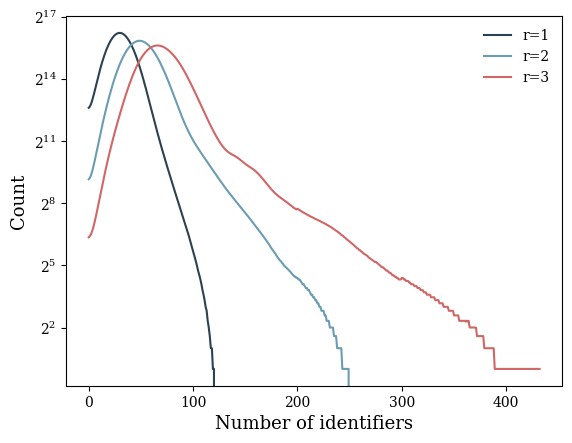
\includegraphics[height=5.4cm]{figures/num_bits}
    \end{subfigure}%
    ~
    \begin{subfigure}[!t]{0.5\textwidth}
        \centering
        b) The hydrocarbon dataset
        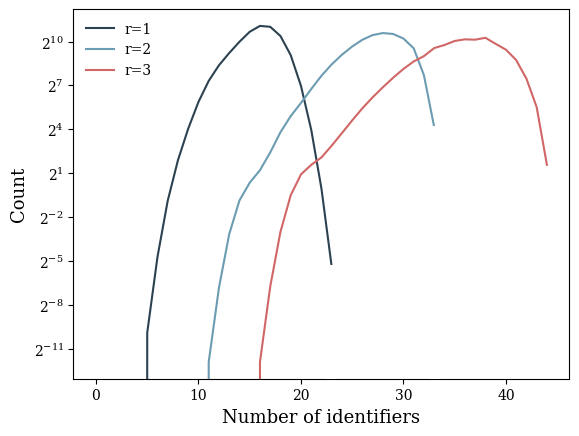
\includegraphics[height=5.4cm]{figures/num_bits_c22}
    \end{subfigure}
    \caption{Number of identifiers generated in the ECFP procedure}
    \label{fig:num_bits}
\end{figure}

The longest encoding for \( r=3 \), in the random dataset, contained \( 432 \) identifiers. As expected, the~encodings of the set of hydrocarbons had a distribution more concentrated around the~mean, as~the range of the number of identifiers was between \( 9 \) and \( 45 \). Comparing the results to~the length of the encoding \( N \approx 10^3 \), the~representation is sparse -- even more so in the average case and for smaller \( r \). Despite this, when projecting identifiers onto a~binary vector of a fixed length some collisions may occur.
\begin{figure}[H]
    \centering
    a) The random dataset
    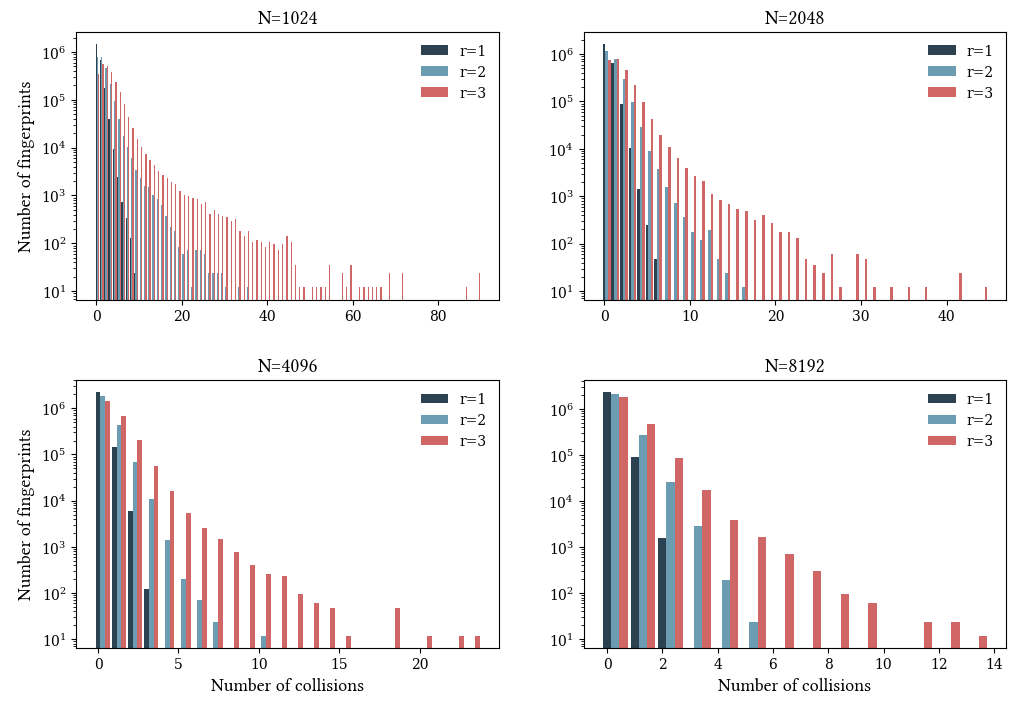
\includegraphics[width=0.95\textwidth]{figures/num_collisions.png}
\end{figure}
\begin{figure}[H]
    \centering
    b) The hydrocarbon set
    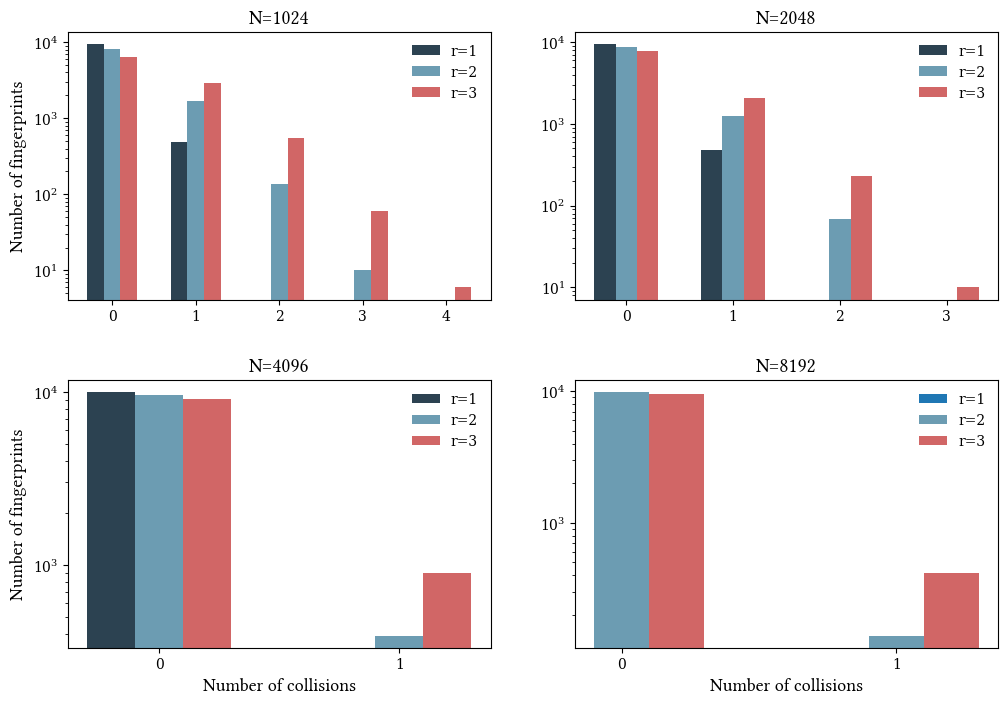
\includegraphics[width=0.95\textwidth]{figures/num_collisions_c22.png}
    \caption{Number of~collisions due to~projection of~identifiers on a~vector depending on the~parameters \( r,\; N \) for a) random set b) hydrocarbon family}
    \label{fig:num_collisions}
\end{figure}
The average number of~collisions for all parameter configurations was less than 3, and for \( r=1 \) or for \( N \geq 4096 \) it was less than 1. This raises the~question of~how much collisions affect the~similarity coefficient.
\subsection{Effect of~collisions on the~similarity coefficient}
It is possible to~estimate the~effect of~a~single collision on a~value of~the~similarity coefficient.
\begin{propos}
    Given two non-zero encodings \( X \neq Y \),\: let \( x_1, x_2 \) correspond to~identifiers from \( X \) that are projected onto the~same bit. The absolute error for Jaccard similarity of~\( X \) and \( Y \) is at most \( \frac{1}{|X \cup Y| - 1} \).
\end{propos}
\begin{proof}
    The similarity coefficient is defined as~\( s(X,Y) = \frac{|X \cap Y|}{|X \cup Y|} \), where \( \abs{X \cup Y} \geq 2 \), thus after the~reduction at least one bit is set. Let \( \tilde{s}(X,Y) \) denote the~Jaccard similarity coefficient of~the~encodings of~\( X \) and \( Y \) with a~single collision of~the~bits \( x_1,\; x_2 \). There are three cases to~consider:
    \begin{itemize}
        \item \( x_1, x_2 \notin X \cap Y \): \\
        The value of~\( |X \cap Y| \) does not change because \( x_1, x_2 \) remain outside the~intersection and the~value of~\( |X \cup Y| \) decreases by \( 1 \).
        \[
            \abs{s(X,Y) - \tilde{s}(X,Y)} = \abs{\frac{|X \cap Y|}{|X \cup Y|} - \frac{|X \cap Y|}{|X \cup Y|-1}} = \frac{|X \cap Y|}{|X \cup Y|(|X \cup Y|-1)} \leq \frac{1}{|X \cup Y| - 1}
        \]
        This gives an absolute error of \( \frac{1}{|X \cup Y|-1} \).
        
        \item \( x_1 \in X \cap Y,\; x_2 \notin X \cap Y \): \\
         In this case, the~value of~\( |X \cap Y| \) also doesn't change because initially only \( x_1 \) contribute to~\( |X \cap Y| \). The value of~\( |X \cup Y| \) again decreases by \( 1 \). The result is therefore the~same as~for the~previous case.
         
        \item \( x_1, x_2 \in X \cap Y \): \\
        Both \( |X \cap Y| \) and \( |X \cup Y| \) decrease.
        \[
            \abs{s(X,Y) - \tilde{s}(X,Y)} = \abs{\frac{|X \cap Y|}{|X \cup Y|} - \frac{|X \cap Y|-1}{|X \cup Y|-1}} = \frac{|X \cup Y|-|X \cap Y|}{|X \cup Y|(|X \cup Y|-1)} < \frac{1}{|X \cup Y|-1}
        \]
        This gives an absolute error of at most \( \frac{1}{|X \cup Y|-1} \).
    \end{itemize}
\end{proof}
For single collisions, their effect on the~value of~the~Jaccard similarity coefficient is rather small, although they may strongly influence the~results of~searching for structures at a~fixed similarity cut-off. Minimising the~inaccuracy by choosing a~sufficiently large \( N \) increases the~sparsity of~the~representation, the~problem to~be solved.

% Chatper II
\chapter{Numerical representation}
\section{Variable-length representation}
\subsection{Data structure for representing fingerprints}
The straightforward solution to the problem of~sparsity is to store all generated identifiers in~a~structure of variable size. No information is lost, and the size of~the structure is at most \( (r+1) \) times the number of~vertices, so in the average case it is smaller than the standard fingerprint length. This makes such a~representation implementable in real-life cases. \\
The designed structure should allow:
\begin{itemize}
\singlespacing
    \item iteration over identifiers,
    \item checking whether the encoding contains a~given identifier,
    \item fast calculation of~the Jaccard similarity coefficient (i.\:e. the size of~intersection and union of~the sets of~identifiers) for two structures of~this type.
\end{itemize}
The main solution commonly used is to store an array of~sorted identifiers \cite{chemaxon2025docs}. Any specified value can be retrieved in time \( \bigO(\log n) \) using binary search.


\subsection{Time complexity of~calculating similarity coefficient}
The union and intersection for two sets of~size \( n_1,\; n_2 \) stored as sorted arrays can be determined at time \( \bigO(n_1 + n_2) \) using the two-pointer method. As the calculation of~the similarity coefficient involves only the size of~the union and the intersection, its value can be determined faster. For this purpose, an exponential search can be used combined with a~binary search.
\begin{algorithm}[H]
    \caption{Computing Jaccard similarity}
    \label{alg:data_struct}
    \begin{algorithmic}[1]
        \Require{\( X\in \real^{n_1},\;Y \in \real^{n_2} \) sorted}
        \Ensure{\( s(X,Y) \)}
        \State \( common \gets 0,\; index \gets 0 \)
        \For {\( x \) \in \( X \)}
        \State \( l \gets index,\; r \gets l + 1 \)
        \While {\( r < n_2 \) and \( Y[r] < x \)}
        \State \( l \gets r,\; r \gets 2 \cdot r \)
        \EndWhile
        \State \( new\_index \gets \text{binSearch}(Y, x, l, r) \)
        \If{\( new\_index \neq -1 \)}
        \State \( common \gets common + 1,\; index \gets new\_index + 1 \)
        \Else
        \State \( index \gets r \)
        \EndIf
        \EndFor
        \State \( s \gets common \;/\; (n_1 + n_2 - common) \)
        \State \Return \( s \)
    \end{algorithmic}
\end{algorithm}
\begin{propos}
    Given two ECFP fingerprints \(X,\; Y\) stored as described above, such that \( X,\; Y \) have sizes respectively \( n_1,\; n_2 \), where \( n_1 \leq n_2 \), then \( s(X,Y) \) can be calculated in \( \bigO(n_1 + n_1\log\frac{n_2}{n_1}) \) time complexity.
\end{propos}
\begin{proof}
    Iterating over the values of~\( X \), we try to match elements in \( Y \). We perform a~binary search to find the index in Y to which we should jump. In total, this requires \( \bigO\!\pars{\sum_{i=1}^{n_1}\; \log x_i } \) comparisons, where \( x_i \) is the length of~the \( i \)-th jump and \( x_1 + \dots + x_{n_1} = n_2 \). From the inequality between the arithmetic and geometric mean, it follows that
    \[
        \sum_{i=1}^{n_1}\; \log x_i = \log\pars{\prod_{i=1}^{n_1}\; x_i} \leq \log\pars{\ceil{\frac{n_2}{n_1}}^{n_1}} = n_1\log\!\ceil{\frac{n_2}{n_1}},
    \]
    which gives time complexity \( \bigO\!\pars{n_1 + n_1\log\frac{n_2}{n_1}} \).
\end{proof}
Potential improvements to this complexity involve better use of~memory or parallelization of~calculations. In practice, however, the size of~the arrays is at most the order of \( 10^3 \), so further optimisations are not needed.

\section{Fixed-length representation}
Fixed-length representations enable efficient storage of multidimensional numerical data. This property can simplify computations and is required for the input of certain classes of machine-learning models. However, reducing the dimensionality of the encodings inevitably causes some information loss, in particular a dictionary-like indication of the presence of a specific substructure. It may still be possible to retain enough information to preserve pairwise similarity between objects. Specifically for the case of ECFP encodings of a set of chemical compounds, the potential solutions are the Johnson-Lindenstrauss and MinHash methods. They let project numerical data into a lower-dimensional space while preserving pairwise distances with high probability.

\subsection{Johnson-Lindenstrauss reduction}
Johnson-Lindenstrauss method is used to project a numerical or binary vectors of a fixed length into a smaller dimension while preserving the pairwise Euclidean distance. The position of points in space can thus reflect the similarity between them. The correctness of the method is based on the following lemma.
\begin{lemma}[Johnson–Lindenstrauss, \( 1984 \) \cite{ghojogh2021lj, weinberg2019lj}]
\label{lemma:JL}
For a fixed \( 0 < \eps < 1 \) and a set of \( m \) points \( \mathcal{X} \subset \real^N \) there exists linear mapping \( f\!:\real^N \rightarrow \real^n \), where \( n = \Omega(\log(m)\eps^{-2}) \), satisfying
\[
    (1-\eps)\:\norm{u-v}^2 \leq \norm{f(u)-f(v)}^2 \leq (1+\eps)\:\norm{u-v}^2
\]
for all \( u,\; v \in \mathcal{X} \).
\end{lemma}
\begin{proof}
Let \( A \in \real^{n \times N} \) be a matrix such that \( a_{ij} \sim \mathcal{N}(0,1) \). Defining a projection \( \Pi = \frac{1}{\sqrt{n}}A \), \linebreak we prove that \( \Pi x \) approximates the norm of \( x \).
\[
    \norm{\Pi x}^2 = \left\|\frac{1}{\sqrt{n}}Ax\right\|^2 = \frac{1}{n} \sum_{i=1}^n\: (a_ix)^2
\]
The values \( a_{ij} \) are sampled at random from the distribution \( \mathcal{N}(0,1) \), so \( x_j a_{ij} \) is also a random variable.
\[
    \mathbb{E}\brackets{a_ix} = \mathbb{E}\brackets{\sum_{j=1}^N x_ja_{ij}} = \sum_{j=1}^N x_j\cdot \mathbb{E}\brackets{a_{ij}} = 0
\]
\[
    \mathbb{E}\brackets{(a_ix)^2} = \operatorname{Var}[a_ix] = \sum_{j=1}^N \operatorname{Var}[a_{ij}x_j] = \sum_{j=1}^N x_j^2 \operatorname{Var}[a_{ij}] = \sum_{j=1}^N x_j^2 = \norm{x}^2.
\]
Hence, the expected norm of \( x \) after the projection is equal to the initial norm:
\[
    \mathbb{E} \brackets{\: \norm{\Pi x}^2 \:} = \mathbb{E} \brackets{\frac{1}{n} \sum_{i=1}^n\: (a_ix)^2} = \norm{x}^2
\]
The random variable \( a_ix \sim \mathcal{N}(0, \norm{x}^2) = \norm{x}\cdot \mathcal{N}(0, 1) \) is concentrated around the mean, so the approximation does not deviate significantly from the expected value. For \( y = \norm{\Pi x} \), by applying the Chernoff inequality we obtain:
\[
    \Pr \brackets{\abs{\mathbb{E}y - y} \geq \eps \cdot \mathbb{E}y} \leq 2 e^{-n \eps^2 / 8}
\]
For \( n = \Omega(\log(1/\delta)\eps^{-2}) \), the inequality:
\[
    (1-\eps)\norm{x}^2 \leq \norm{\Pi x}^2 \leq (1+\eps)\norm{x}^2
\]
is satisfied with probability at least \( (1-\delta) \). \\
Substituting \( x \) with \( u-v \), we obtain the proof that the Johnson-Lindenstrauss reduction almost preserves Euclidean distance between any pair of vectors from \( \mathcal{X} \). Since there are \( {m \choose 2} \) pairs of points, from the linearity of expectation, all distances are preserved within error \( \eps \) with probability at least \( (1-\delta) \) if we assume \( n = \Omega(\log(m/\delta)\eps^{-2}) \).
\end{proof}
The proof is constructive and the defined projection can be easily implemented according to~the following steps:
\begin{algorithm}[H]
    \caption{Johnson-Lindenstrauss reduction}
    \label{alg:jl}
    \begin{algorithmic}[1]
        \Require{\( n \in \mathbb{N},\; x \in \real^N \)}
        \Ensure{\( x' \in \real^n \)}

        \State Initialize \( A \in \real^{n \times N} \)
        \For{\( i \in \set{0, \dots, n-1} \)}
        \For{\( j \in \set{0, \dots, N-1} \)}
        \State \( A[i][j] \gets \mathcal{N}(0,1) \)
        \EndFor
        \EndFor
        \State \( \Pi \gets \frac{1}{\sqrt{n}}A \)
        \State \Return \( \Pi x \)
    \end{algorithmic}
\end{algorithm}

The transformation can be performed in time \( \bigO(m \cdot Nn) = \bigO(m \cdot N \: \log(m/\delta)\eps^{-2}) \) for a set of \( m \) vectors, that is, polynomial in terms of size of \( \mathcal{X} \) and the initial length of encoding, which in this case is a constant of order \( 10^3 \). Hence, for large sets of compounds it holds that \( m >\!\!> N \). The time complexity of multiplication of matrix \( A \) with a vector \( u \) can be improved to~\( \Theta(k \cdot \| u \|_0) = \bigO(n \cdot N) \), where \( k \) denotes the maximum support of columns of matrix \( A \)~\cite{freksen2021jl}. Different variants of the transformation \( f \) have been developed that satisfy the Johnson-Lindenstrauss lemma and improve time complexity. For example, the Fast Johnson-Lindenstrauss Transform, which uses a sparse projection matrix, achieves \( \bigO(N \log N) \) time complexity in the general case, while Ailon and Liberty reduced it to \( \bigO(N \log n) \) when \( n = \bigO(N^{1/2 - \gamma}) \) for a fixed constant \( \gamma > 0 \) \cite{freksen2021jl}.


It remains to show that the Johnson-Lindenstrauss lemma can be generalised to another distance metric.
\begin{propos}
    The Johnson-Lindenstrauss lemma is true for Jaccard similarity metric.
\end{propos}
\begin{proof}
The projection \( \Pi \) does not change the expected value of the scalar product, because matrix \( A^TA \) is usually close to the unit matrix.
\[
    \mathbb{E} \brackets{(A^TA)_{ij}} = \sum_{k=1}^{n} \mathbb{E} \brackets{a_{ki} \cdot a_{kj}} = \sum_{k=1}^{n} \one\!\brackets{i = j} = n \cdot \one\!\brackets{i = j}
\]
\[
    \mathbb{E}\brackets{\dotpr{\Pi u, \Pi v}} = \mathbb{E}\brackets{\dotpr{\frac{1}{\sqrt{n}} Au, \frac{1}{\sqrt{n}} A v}} = \frac{1}{n}\mathbb{E} \brackets{u^TA^TAv} = \frac{1}{n} u^T \cdot \mathbb{E} \brackets{A^TA} \cdot v = u^Tv,
\]
The inequality
\[
    (1-\eps)\:\norm{u-v}^2 \leq \norm{f(u)-f(v)}^2 \leq (1+\eps)\:\norm{u-v}^2,
\]
follows from the Lemma~\ref{lemma:JL}. Now, it is needed to prove that the inequality also holds for the scalar product. The useful identities are: \\
Parallelogram law:
\[
    \norm{x+y}^2 + \norm{x-y}^2 = 2\norm{x}^2 + 2\norm{y}^2
\]
Polarisation identity:
\[
    \dotpr{x, y} = \frac{1}{4} \pars{\norm{x+y}^2 - \norm{x-y}^2}
\]
It follows that:
\[
    \dotpr{f(u), f(v)} = \frac{1}{4}\pars{\norm{f(u)+f(v)}^2 - \norm{f(u)-f(v)}^2} \geq \frac{1}{4}\pars{(1-\eps)\norm{u+v}^2 - (1+\eps)\norm{u-v}^2}
\]
\[
    = \frac{1}{4}\pars{\norm{u+v}^2 - \norm{u-v}^2} - \frac{1}{4}\eps\pars{\norm{u+v}^2 + \norm{u-v}^2} = \dotpr{u,v} - \frac{1}{2}\eps\pars{\norm{u}^2 + \norm{v}^2}
\]
To complete the proof, an additional observation is needed:
\begin{lemma}
    The Jaccard similarity is not affected by positive scalar multiplication.
\end{lemma}
\begin{proof}
    Let \( c \in \real^{+} \), then:
    \[
        s(cu, cv) = \frac{\dotpr{cu, cv}}{\norm{cu}^2 + \norm{cv}^2 - \dotpr{cu, cv}}  = \frac{c^2 \dotpr{u, v}}{c^2\pars{\norm{u}^2 + \norm{v}^2} - c^2 \dotpr{u, v}} = \frac{\dotpr{u, v}}{\norm{u}^2 + \norm{v}^2 - \dotpr{u, v}} = s(u, v)
    \]
\end{proof}
\noindent
We can now assume that the binary fingerprints of length \( N \) have norm at most 1, since they can be multiplied by \( \frac{1}{\sqrt{N}} \), and then the dot product is bounded by:
\[
    \dotpr{f(u), f(v)} \geq \dotpr{u,v} - \frac{1}{2}\eps\pars{\norm{u}^2 + \norm{v}^2} \geq \dotpr{u,v} - \eps
\]
This proves the inequality:
\[
    (1-\eps) \dotpr{u,v} \leq \dotpr{f(u), f(v)} \leq (1+\eps)\dotpr{u,v}
\]
The formula for Jaccard similarity is:
\[
    s(f(u), f(v)) = \frac{\dotpr{f(u), f(v)}}{\norm{f(u)} + \norm{f(v)} - \dotpr{f(u), f(v)}} = \frac{\dotpr{f(u), f(v)}}{\norm{f(u)-f(v)} + \dotpr{f(u), f(v)}},
\]
which can be derived using the parallelogram law and the polarisation identity:
\[
    \norm{f(u)} + \norm{f(v)} - \dotpr{f(u), f(v)} = \frac{1}{2} \pars{\norm{f(u) + f(v)}^2 + \norm{f(u) - f(v)}^2} - \dotpr{f(u), f(v)}
\]
\[
    = \frac{1}{2} \pars{4\dotpr{f(u), f(v)} + 2\norm{f(u) - f(v)}^2} - \dotpr{f(u), f(v)} = \dotpr{f(u), f(v)} + \norm{f(u) - f(v)}^2
\]
Plugging the above results for \( 0 < \eps \leq \frac{1}{2} \) into the formula for Jaccard similarity gives:
\[
    s(f(u), f(v)) \leq \frac{\dotpr{u, v} \cdot (1+\eps)}{\pars{\norm{u-v} + \dotpr{u, v}} \cdot (1-\eps)} = s(u, v) \cdot \pars{1 + \frac{2\eps}{1-\eps}} \leq s(u, v) \cdot (1 + 4\eps)
\]
\[
    s(f(u), f(v)) \geq \frac{\dotpr{u, v} \cdot (1-\eps)}{\pars{\norm{u-v} + \dotpr{u, v}} \cdot (1+\eps)} = s(u, v) \cdot \pars{1 - \frac{2\eps}{1+\eps}} \leq s(u, v) \cdot (1 - 2\eps)
\]
It shows that for \( n \in \Omega(\log(m/\delta)\eps^{-2}) \) the Jaccard similarity satisfies
\[
    (1-\eps) \cdot s(u,v) \leq s(f(u), f(v)) \leq (1+\eps) \cdot s(u,v)
\]
\end{proof}
\subsection{MinHash reduction}
Unlike the previous method, MinHash can be applied to both fixed and variable length vectors. The input vectors can be numerical or binary, but the latter requires transforming them into a set of non-zero indices. The advantage of the MinHash method is that it directly preserves the Jaccard similarity. Thus, the MinHash method is well suited to convert the list of identifiers returned by the ECFP algorithm directly into a fixed-length encoding without previously projecting it into a~vector. \\
To present the MinHash reduction, first, a few definitions are needed \cite{broder1997resemblance, musco2020minhash}. For a fixed \( k \in \mathbb{N} \) and a set \( X \subseteq \Omega \) with given ordering corresponding to a random permutation of \( \Omega \), define:
\[
    \text{min}_k(X) = \set{x_i \in X : 1 \leq i \leq \min\set{k, \abs{X}}}
\]
Then, the similarity of sets \( X, Y \subseteq \Omega \) can be expressed as:
\[
    s_k(X,Y) = \frac{\abs{\text{min}_k(X \cup Y) \cap \text{min}_k(X) \cap \text{min}_k(Y)}}{\abs{\text{min}_k(X \cup Y)}}
\]
With the above definitions in hand, it is possible to prove the lemma that is fundamental for the~MinHash method.
\begin{lemma}[\cite{broder1997resemblance}]
    The value of \( s_k(X,Y) \) approximates the Jaccard similarity \( s(X,Y) \).
\end{lemma}
\begin{proof}
    Since the sets \( X \) and \( Y \) are ordered according to a random permutation, each element of~the sets has an equal probability of being the \( i\)-th smallest. For a certain \( x \in \text{min}_k(X \cup Y) \):
    \[
        P(x \in \text{min}_k(X) \cap \text{min}_k(Y)) =  P(x \in  X \cap Y) = \frac{\abs{X \cap Y}}{\abs{X \cup Y}} = s(X,Y)
    \]
\end{proof}

\noindent
By setting \( k = 1 \), the above similarity estimator can be applied to the sets of ECFP identifiers, to derive an implementable algorithm.
\begin{algorithm}[H]
    \caption{MinHash reduction}
    \label{alg:mh}
    \begin{algorithmic}[1]
    \Require{\( n \in \mathbb{N}, \ X \in \real^N \)}
    \Ensure{\( \Tilde{X} \in \real^n \)}
        \State define uniform hashing functions \( h_1, \dots, h_n: \real \rightarrow [0,1] \)
        \State \( f(X)_i \gets \min_{x \in X}\: h_i(x) \)
        \State \Return \( \brackets{\:f(X)_1, \dots, f(X)_n\:} \)
    \end{algorithmic}
\end{algorithm}
\noindent
The algorithm has time complexity \( \bigO(Nn) \). It can be proven to preserve the Jaccard similarity with high probability.
\begin{propos}[\cite{broder1997resemblance, musco2020minhash}]
\label{propos:MH}
For \( 0 < \eps < 1 \) and \( n = \bigO(\log(m/\delta)\eps^{-2}) \), the Jaccard similarity of \( X,\;Y \) transformed using the MinHash method 
\(
    s(f(X),f(Y)) = \frac{1}{n} \sum_{i=1}^{n}\; \mathbbm{1}\!\brackets{f(X)_i = f(Y)_i}
\)
satisfies
\[
    s(X,Y) - \eps \leq s(f(X),f(Y)) \leq s(X,Y) + \eps
\]
for any \( X \in \real^{N_1},\; Y \in \real^{N_2} \).
\end{propos}
\begin{proof}
The estimator \( s(f(X),f(Y)) \) is unbiased, because \( \mathbb{E}\brackets{\: \mathbbm{1}\!\brackets{f(X)_i = f(Y)_i} \:} = s(X,Y) \). \\
The inaccuracy of approximation can be bounded by applying Hoeffding inequality:
\[
    P\pars{\abs{s(f(X),f(Y)) - s(X,Y)} \geq \eps} \leq 2e^{-2n\eps^2}
\]
It simply follows that for some \( X \) and  \( Y \), and \( n = \bigO(\log(1/\delta)\eps^{-2}) \) with probability at least \( (1-\delta) \) it is true that
\[
    s(X,Y) - \eps \leq s(f(X), f(Y)) \leq s(X,Y) + \eps
\]
Therefore, from the linearity of expectation, the similarity is preserved for all possible pairs of~vectors when \( n = \Omega(\log(m/\delta)\eps^{-2}) \).
\end{proof}

% Chatper III
\chapter{Applications}
\section{Effect of dimension reduction on pairwise similarity}
The Johnson-Lindenstrauss and MinHash methods have been implemented (see~\hyperref[ch:appendix]{Appendix}) and tested on a set of \( 1000 \) compounds randomly selected from the original datasets using the bash terminal \texttt{shuf} command. The parameters used for the analysis were \( r = 3 \) and \( N \in \set{128, 512, 2048} \), so \( N \sim \log(m)\epsilon^{-2} \) for \( m = 1000 \) and \( 0.05 \leq \epsilon \leq 0.25 \).

The goal of the experiment was to compare the approaches to dimensionality reduction of~the encodings, by evaluating how well each method preserved the pairwise similarity between the compounds. The Johnson-Lindenstrauss and MinHash methods were compared to manipulating the length of the fingerprints modulo the value of \( N \). The \autoref{fig:reduced} shows how the distribution of distances in the Jaccard metric has changed for the studied methods.
\begin{figure}[H]
    \centering
    a) The random dataset
    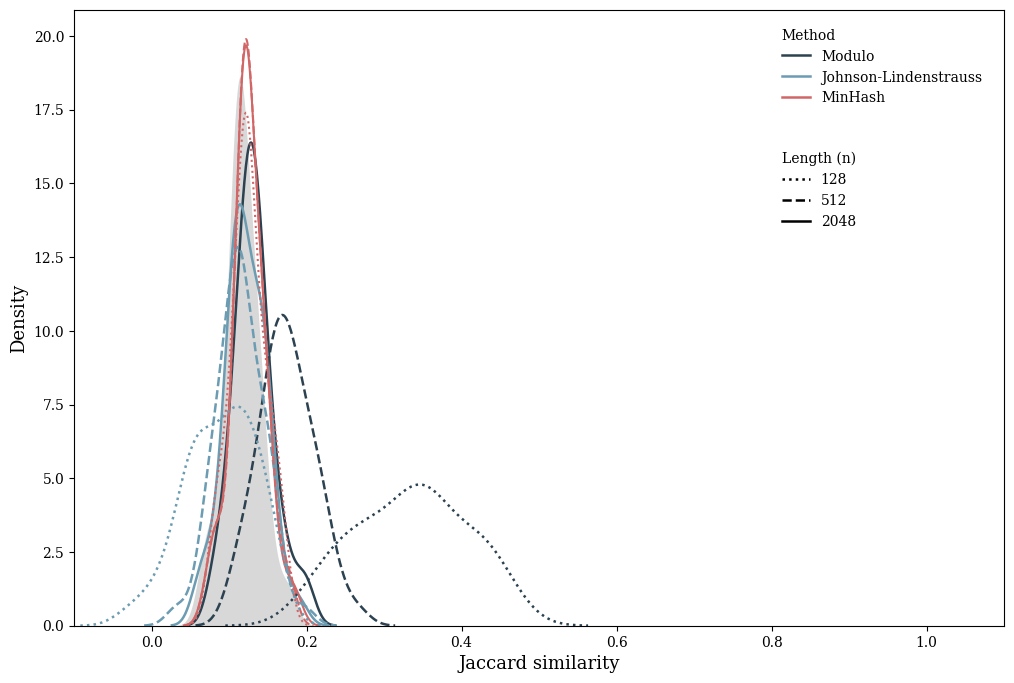
\includegraphics[width=0.8\textwidth]{figures/reduced.png}
\end{figure}
\begin{figure}[H]
    \centering
    b) The hydrocarbon dataset
    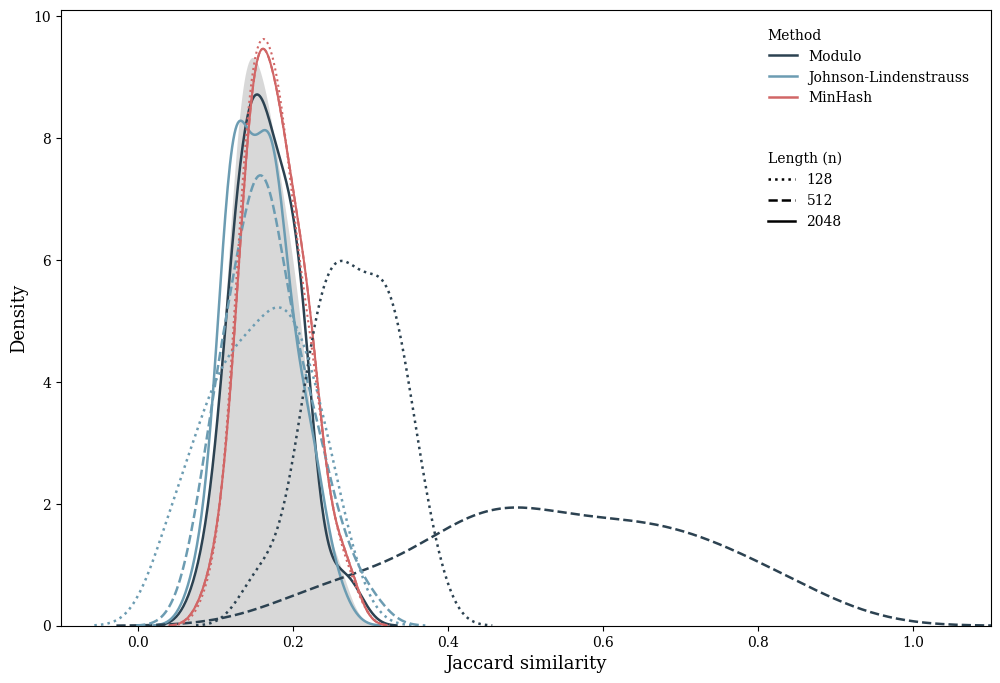
\includegraphics[width=0.8\textwidth]{figures/reduced_c22.png}
    \caption{Distribution of distance in Jaccard metric for the encodings reduced with different methods}
    \label{fig:reduced}
\end{figure}
For the original non-reduced fingerprints from the random dataset, Jaccard distance ranged from \( 0.871 \) to \( 0.985 \) with a mean of \( 0.933 \). For \( N = 8192 \), the distributions of distances for reduced encodings did not differ much from the original distributions. For smaller values of \( N \), however, the Johnson-Lindenstrauss and MinHash methods outperformed the naive method. Reducing the fingerprint length modulo \( N \) lead to visibly broadened distribution. For \( N = 128 \), the mean distance was equal to \( 0.715 \) with the most similar pair of compounds having distance of \( 0.587 \). For both other methods, the absolute difference in pairwise distance compared to the original one in no case exceeded \( 0.10 \) for the Johnson-Lindenstrauss and \( 0.03 \) for the MinHash reduction.

\section{Effect of dimension reduction on KNN-search accuracy}
Cluster analysis and similarity search play a crucial role in identifying patterns in molecular structures and predicting their properties. Consequently, they are among the most commonly used methods of \emph{in silico} studies exploring the structure-activity relationship of chemical compounds. In such context, under the assumption that the similarity between compounds is proportional to~the similarity of their numerical representation, the similarity search can be effectively performed as a KNN-search in the feature space \cite{weber1998knn}. This process is computationally expensive, particularly when operating on high-dimensional representations such as molecular fingerprints. The nearest neighbour similarity search, therefore, serves as an apt validation test for the practical applicability of dimensionality reduction techniques like Johnson-Lindenstrauss and MinHash, which aim to~reduce computational costs without sacrificing accuracy.

The goal is to reduce the likelihood of a false negative, i.e. rejecting a potential neighbour that would be selected based on the original, non-reduced encoding. An error of this kind is more costly than a false positive because it excludes from further study a compound that could potentially be~a~good candidate for the desired active ingredient. The assumption is that the nearest-neighbour search method itself does not use an approximation algorithm and always returns the correct result. In addition, in the context of this problem, instead of similarity, the Jaccard distance (see~\hyperref[ch:notation]{Notation}) will be used, which is directly related to the similarity and follows the convention used for the KNN search. This analysis refers to the MinHash reduction, which has proven to be~the best experimentally and has the desired theoretical properties.

For the analysis, the Jaccard distance distribution for the random set and hydrocarbons can be modelled with a normal distribution.
\begin{figure}[H]
    \centering
    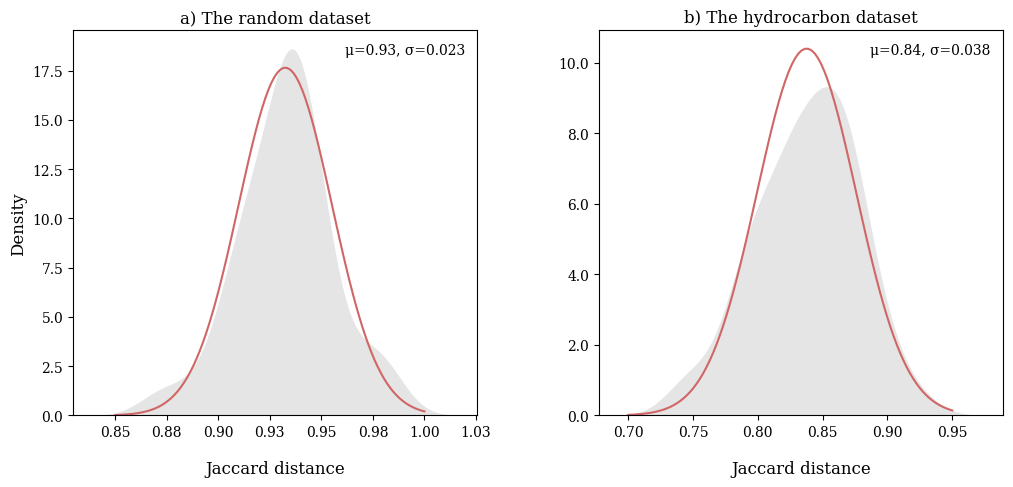
\includegraphics[height=6cm]{figures/similarity_distributions_only.png}
    \caption{Fit of normal distribution to distribution of Jaccard distance}
    \label{fig:normal}
\end{figure}
The problem has two variants: searching for exactly \( k \) nearest neighbours or searching for all neighbours with a distance of at most \( k \) from the input structure. Let \( E \) be an event that a vector \( v \) is included in the results of the search based on the original encoding, and let \( \tilde{E} \) denote the event that \( \tilde{v} = f(v) \) is included in the results of the search based on the reduced encoding. Let \( u \) be the encoding of a given input structure. Suppose we search in a set of \( m \) structures with \( N \) being the maximum number of identifiers generated by the ECFP algorithm. The reduced encoding has length \( n = \bigO(\log(m)\eps^{-2}) \), as in the Lemma~\ref{propos:MH}.

\subsection{Search with fixed distance threshold}
We are given the initial structure \( u \) and the distance threshold \( 0 < k < 1 \). The probability of~observing a false negative is:
\[
    P(\neg \tilde{E} \mid E) = P(d(\tilde{u}, \tilde{v}) > k \mid d(u, v) \leq k)
\]
Since the size of the set of ECFP identifiers for each structure is limited linearly from the size of the structure, the distances between structures take on values from a specific discrete range \linebreak \( D \subseteq \set{\frac{\abs{u \:\cap\: v}}{\abs{u \:\cup\: v}} \colon 0 \leq \abs{u \cap v} \leq N,\; 0 < \abs{u \cup v} \leq 2N} \). Hence, the above probability can be bounded by iterating over all possible distances between \( u \) and \( v \) that are not greater than \( k \):
\[
    P(\neg \tilde{E} \mid E) = \sum_{d_i \in D,\; d_i \leq k}\; P(d(\tilde{u}, \tilde{v}) > d(u, v) + (k - d_i) \mid d(u, v) = d_i) \cdot P(d(u, v) = d_i)
\]
For the MinHash method, we can bound the probability using the Proposition~\ref{propos:MH} and the fact that the distribution of Jaccard distance can be approximated using a normal distribution \( \mathcal{N}(\mu, \sigma^2) \) fitted for the used datasets, to obtain:
\[
    P(\neg \tilde{E} \mid E) \leq \sum_{d_i \in D}\; 2e^{-n(k-d_i)^2} \cdot \frac{1}{\sqrt{2 \pi} \sigma} e^{-\frac{(d_i - \mu)^2}{2\sigma^2}} = \sum_{d_i \in D}\; 2e^{-n(k-d_i)^2} \cdot \frac{1}{\sqrt{2 \pi} \sigma} e^{-\frac{(d_i - \mu)^2}{2\sigma^2}} 
\]
\[
    = \sqrt{\frac{2}{\pi\sigma^2}} \cdot \sum_{d_i \in D}\; e^{-n(k-d_i)^2-\frac{(d_i - \mu)^2}{2\sigma^2}}
\]
The results obtained experimentally and averaged over 1000 trials are presented in \autoref{tab:knn-distance}.
\begin{table}[ht]
    \centering
    \begin{subtable}[t]{0.45\textwidth}
        \centering
        \caption{The random dataset}
        \begin{tabular}{lccc}
            \toprule
            \( k \) & \( n = 128 \) & \( n = 512 \) & \( n = 2048 \) \\
            \midrule
            0.5 & 0.002 & \( < 0.001 \) & \( < 0.001 \) \\
            0.6 & 0.010 & 0.002 & \( < 0.001 \) \\
            0.7 & 0.033 & 0.001 & \( < 0.001 \) \\
            0.8 & 0.177 & 0.008 & \( < 0.001 \) \\
            0.9 & 0.203 & 0.008 & \( < 0.001 \) \\
            \bottomrule
        \end{tabular}
    \end{subtable}%
    \hfill
    \begin{subtable}[t]{0.45\textwidth}
        \centering
        \caption{The hydrocarbon dataset}
        \begin{tabular}{lccc}
            \toprule
            \( k \) & \( n = 128 \) & \( n = 512 \) & \( n = 2048 \) \\
            \midrule
            0.5 & 0.008 & \( < 0.001 \) & \( < 0.001 \) \\
            0.6 & 0.057 & \( < 0.001 \) & \( < 0.001 \) \\
            0.7 & 0.069 & \( < 0.001 \) & \( < 0.001 \) \\
            0.8 & 0.034 & \( < 0.001 \) & \( < 0.001 \) \\
            0.9 & 0.001 & \( < 0.001 \) & \( < 0.001 \) \\
            \bottomrule
        \end{tabular}
    \end{subtable}
    \caption{Experimental false positive rate in KNN depending on the distance threshold \( k \)}
    \label{tab:knn-distance}
\end{table}


\subsection{Search with fixed number of results}
We are given the initial structure \( u \) and the searched number of nearest neighbours \( k \). Let \( E_j \) represent the probability that \( v \) is the \( j \)-th nearest neighbour of \( u \). The probability of observing a false negative is:
\[
    P(\neg \tilde{E} \mid E) = \frac{P(\neg \tilde{E} \land E)}{P(E)} =  \frac{1}{P(E)} \sum_{j \in [k]} P(\neg \tilde{E} \land E_j)
\]
This can be approximated by the probability that there are at least \( k-j \) vectors that are further from \( u \) than \( v \) when non-reduced but closer after the transformation. For a vector \( v_i \) satisfying the above condition, let \( d_v,\; d_{v_i} \) be respectively the distances of \( v \) and \( v_i \) from \( u \). Let \( d_{uv} \) denote the distance by which \( v \) moves relative to \( u \), that is \( d_{uv} = \abs{d(u, v) - d(\tilde{u}, \tilde{v})} \). The following scenarios are possible:
\begin{itemize}
    \item If \( d(u, v) \leq d(\tilde{u}, \tilde{v}) \) and \( d(u, v_i) \leq d(\tilde{u}, \tilde{v_i}) \), the distance of \( v_i \) from \( u \) must decrease by at~least \( d_{v_i} - d_v + d_{uv} \):
    \[
        P(\abs{d(u, v_i) - d(\tilde{u}, \tilde{v_i})} \geq d_{v_i} - d_v + d_{uv}) \leq 2 e^{-n(d_{v_i} - d_v + d_{uv})^2}
    \]
    \item If \( d(u, v) > d(\tilde{u}, \tilde{v}) \) and \( d(u, v_i) \geq d(\tilde{u}, \tilde{v_i}) \), the distance of \( v_i \) from \( u \) must decrease by at~least \( d_{v_i} - d_v - d_{uv} \):
    \[
        P(\abs{d(u, v_i) - d(\tilde{u}, \tilde{v_i})} \geq d_{v_i} - d_v - d_{uv}) \leq 2 e^{-n(d_{v_i} - d_v - d_{uv})^2}
    \]
    \item If \( d(u, v) > d(\tilde{u}, \tilde{v}) \) and \( d(u, v_i) > d(\tilde{u}, \tilde{v_i}) \), the distance of \( v_i \) from \( u \) must decrease by at~most \( d_{v_i} - d_v + d_{uv} \):
    \[
       P(\abs{d(u, v_i) - d(\tilde{u}, \tilde{v_i})}) \leq d_{v_i} - d_v + d_{uv}) \leq 1 - 2 e^{-n(d_{v_i} - d_v + d_{uv})^2}
    \]
\end{itemize}
Combining the above, and given \( d_v \), \( d_{v_i} \) and \( d_{uv} \), the probability that the transformation introduced an inversion between \( v \) and \( v_i \) with respect to the distance to \( u \) can be bounded by:
\[
    2 e^{-n(d_{v_i} - d_v + d_{uv})^2} + 2 e^{-n(d_{v_i} - d_v - d_{uv})^2} + 1 - 2 e^{-n(d_{v_i} - d_v + d_{uv})^2} = 2 e^{-n(d_{v_i} - d_v - d_{uv})^2} + 1
\]
Summing over the possible values of \( d_v \), \( d_{v_i} \) and \( d_{uv} \), we obtain the bound:
\[
    P(d(u, v) < d(u, v_i) \land d(\tilde{u}, \tilde{v}) > d(\tilde{u}, \tilde{v_i})) \leq
\]
\[
    \leq \sum_{d_v \leq d_{v_i} \in D} \pars{P(d(u,v) = d_v, \ d(u, v_i) = d_{v_i}) \cdot \sum_{d_v \in D} P(\abs{d(u, v) - d(\tilde{u}, \tilde{v})} = d_{uv}) \cdot \pars{2 e^{-n(d_{v_i} - d_v - d_{uv})^2} + 1}}
\]
\[
    \leq \sum_{d_v \leq d_{v_i} \in D} \pars{\frac{1}{2 \pi \sigma^2} e^{-\frac{(d_v - \mu)^2 + (d_{v_i} - \mu)^2}{2 \sigma^2}} \cdot \sum_{d_{uv} \in D} \pars{2e^{-nd_{uv}^2} \cdot \pars{2 e^{-n(d_{v_i} - d_v - d_{uv})^2} + 1}}}
\]
\[
    = \frac{1}{\pi \sigma^2} \cdot\!\!\! \sum_{d_v \leq d_{v_i} \in D} \pars{e^{-\frac{(d_v - \mu)^2 + (d_{v_i} - \mu)^2}{2 \sigma^2}} \cdot \sum_{d_{uv} \in D} e^{-nd_{uv}^2} \cdot \pars{2 e^{-n(d_{v_i} - d_v - d_{uv})^2} + 1}}
\]
To simplify the inner sum, the product can be split into two series of the form \( e^{-x^2} \), and then approximated by a Gaussian integral. Let \( c = d_{v_i} - d_v \) for clarity.
\[
    \sum_{d_{uv} \in D} e^{-nd_{uv}^2} \cdot \pars{2 e^{-n(c - d_{uv})^2} + 1} = \sum_{d_{uv} \in D} e^{-n(c - d_{uv})^2 + d_{uv}^2} + \sum_{d_{uv} \in D} e^{-nd_{uv}^2}
\]
The second sum can be directly approximated by the integral, since for sufficiently large \( N \) the~possible values of \( d_{uv} \) are arranged densely.
\[
    \sum_{d_{uv} \in D} e^{-nd_{uv}^2} \approx \int_{D} e^{-nx^2} dx \leq \int_{0}^{+\infty} e^{-nx^2} dx = \frac{1}{2} \sqrt{\frac{\pi}{n}}
\]
The first sum requires simplification, before a similar approximation can be applied. Because \( c \in [0, 1] \), it follows that:
\[
    \sum_{d_{uv} \in D} e^{-nc^2} \cdot e^{2n\pars{d_{uv}c - d_{uv}^2}} = \sum_{d_{uv} \in D} e^{-nc^2} \cdot e^{n\frac{c^2}{2}} \cdot e^{-2n\pars{d_{uv} - \frac{c}{2}}^2} = e^{-n\frac{c^2}{2}} \cdot \sum_{d_{uv} \in D} e^{-2n\pars{d_{uv} - \frac{c}{2}}^2}
\]
\[
     \approx e^{-n\frac{c^2}{2}} \cdot \int_{D} e^{-n\pars{x - \frac{c}{2}}^2} dx \;\leq\; e^{-n\frac{c^2}{2}} \cdot \int_{0}^{+\infty} e^{-n\pars{x - \frac{c}{2}}^2} dx \;\leq\; \frac{1}{2} e^{-n\frac{c^2}{2}} \cdot  \sqrt{\frac{\pi}{n}}
\]
Applying the above derivation, the consequent result is:
\[
    P(\neg \tilde{E} \land E_j) \leq {m-j \choose k-j} \pars{\frac{1}{\pi \sigma^2} \cdot\!\!\! \sum_{d_v \leq d_{v_i} \in D} \pars{e^{-\frac{(d_v - \mu)^2 + (d_{v_i} - \mu)^2}{2 \sigma^2}} \cdot \sqrt{\frac{\pi}{n}} \cdot e^{-n\frac{(d_{v_i} - d_v)^2}{2}}}}^{k-j}
\]
\[
    = {m-j \choose k-j} \pars{\frac{1}{\sqrt{n \pi} \sigma^2} \cdot\!\!\! \sum_{d_v \leq d_{v_i} \in D} \pars{e^{-\frac{(d_v - \mu)^2 + (d_{v_i} - \mu)^2}{2 \sigma^2}} \cdot e^{-n\frac{(d_{v_i} - d_v)^2}{2}}}}^{k-j}
\]
\\

\noindent
The results obtained experimentally over 1000 trials and different threshold values are presented in \autoref{tab:knn-number}.
\begin{table}[ht]
    \centering
    \begin{subtable}[t]{0.45\textwidth}
        \centering
        \caption{The random dataset}
        \begin{tabular}{lccc}
            \toprule
            \( k \) & \( n = 128 \) & \( n = 512 \) & \( n = 2048 \) \\
            \midrule
            10 & 0.319 & 0.005 & 0.025 \\
            20 & 0.311 & 0.046 & 0.024 \\
            30 & 0.305 & 0.046 & 0.024 \\
            40 & 0.297 & 0.044 & 0.023 \\
            50 & 0.290 & 0.043 & 0.022 \\
            \bottomrule
        \end{tabular}
    \end{subtable}%
    \hfill
    \begin{subtable}[t]{0.45\textwidth}
        \centering
        \caption{The hydrocarbon dataset}
        \begin{tabular}{lccc}
            \toprule
            \( k \) & \( n = 128 \) & \( n = 512 \) & \( n = 2048 \) \\
            \midrule
            10 & 0.152 & 0.020 & 0.020 \\
            20 & 0.139 & 0.019 & 0.019 \\
            30 & 0.135 & 0.022 & 0.021 \\
            40 & 0.129 & 0.023 & 0.023 \\
            50 & 0.126 & 0.022 & 0.022 \\
            \bottomrule
        \end{tabular}
    \end{subtable}
    \caption{Experimental false positive rate in KNN depending on the count threshold \( k \)}
    \label{tab:knn-number}
\end{table}
% RANDOM number threshold
% n=128, k=5) 0.3326
% n=128, k=10) 0.31870000000000004
% n=128, k=15) 0.3150666666666667
% n=128, k=20) 0.31115000000000004
% n=128, k=25) 0.30668000000000006
% n=128, k=30) 0.30466666666666664
% n=128, k=35) 0.30071428571428566
% n=128, k=40) 0.29745
% n=128, k=45) 0.29373333333333335
% n=128, k=50) 0.29041999999999996
% n=1024, k=5) 0.027600000000000003
% n=1024, k=10) 0.025200000000000004
% n=1024, k=15) 0.025333333333333333
% n=1024, k=20) 0.024549999999999995
% n=1024, k=25) 0.023799999999999998
% n=1024, k=30) 0.0243
% n=1024, k=35) 0.024485714285714288
% n=1024, k=40) 0.022925000000000004
% n=1024, k=45) 0.02335555555555555
% n=1024, k=50) 0.02246
% n=8192, k=5) 0.0268
% n=8192, k=10) 0.0247
% n=8192, k=15) 0.025333333333333333
% n=8192, k=20) 0.0243
% n=8192, k=25) 0.023839999999999997
% n=8192, k=30) 0.024166666666666663
% n=8192, k=35) 0.02442857142857143
% n=8192, k=40) 0.022825
% n=8192, k=45) 0.023199999999999995
% n=8192, k=50) 0.02222

% RANDOM distance threshold
% n=128, k=0.1) 0.0
%  n=128, k=0.2) 0.0
%  n=128, k=0.3) 0.0
%  n=128, k=0.4) 0.0
%  n=128, k=0.5) 0.002
%  n=128, k=0.6) 0.01
%  n=128, k=0.7) 0.033083333333333326
%  n=1024, k=0.1) 0.0
%  n=1024, k=0.2) 0.0
%  n=1024, k=0.3) 0.0
%  n=1024, k=0.4) 0.0
%  n=1024, k=0.5) 0.0
%  n=1024, k=0.6) 0.0
%  n=1024, k=0.7) 0.0

% SIMILAR number threshold
%  n=128, k=5) 0.1678
%  n=128, k=10) 0.15180000000000002
%  n=128, k=15) 0.14486666666666667
%  n=128, k=20) 0.13925
%  n=128, k=25) 0.13748000000000002
%  n=128, k=30) 0.13490000000000005
%  n=128, k=35) 0.13174285714285713
%  n=128, k=40) 0.1291
%  n=128, k=45) 0.12848888888888887
%  n=128, k=50) 0.12624000000000002
%  n=128, k=0.1) 0.0
%  n=128, k=0.2) 0.0
%  n=128, k=0.3) 0.0
%  n=128, k=0.4) 0.0
%  n=128, k=0.5) 0.008
%  n=128, k=0.6) 0.057083333333333326
%  n=128, k=0.7) 0.069225093685548
%  n=1024, k=5) 0.0258
%  n=1024, k=10) 0.020200000000000003
%  n=1024, k=15) 0.02053333333333333
%  n=1024, k=20) 0.0189
%  n=1024, k=25) 0.02084
%  n=1024, k=30) 0.021299999999999996
%  n=1024, k=35) 0.021200000000000004
%  n=1024, k=40) 0.022775000000000007
%  n=1024, k=45) 0.021799999999999996
%  n=1024, k=50) 0.02178
%  n=1024, k=0.1) 0.0
%  n=1024, k=0.2) 0.0
%  n=1024, k=0.3) 0.0
%  n=1024, k=0.4) 0.0
%  n=1024, k=0.5) 0.0
%  n=1024, k=0.6) 0.0
%  n=1024, k=0.7) 0.0
%  n=8192, k=5) 0.0258
%  n=8192, k=10) 0.020200000000000003
%  n=8192, k=15) 0.02053333333333333
%  n=8192, k=20) 0.0189
%  n=8192, k=25) 0.02084
%  n=8192, k=30) 0.021299999999999996
%  n=8192, k=35) 0.021200000000000004
%  n=8192, k=40) 0.022775000000000007
%  n=8192, k=45) 0.021799999999999996
%  n=8192, k=50) 0.02178
%  n=8192, k=0.1) 0.0
%  n=8192, k=0.2) 0.0
%  n=8192, k=0.3) 0.0
%  n=8192, k=0.4) 0.0
%  n=8192, k=0.5) 0.0
%  n=8192, k=0.6) 0.0
%  n=8192, k=0.7) 0.0

\section{Effect of dimension reduction on KNN-search time}
The KNN algorithm in a basic implementation has a time complexity of \( \bigO(m \cdot N) \), where \( m \) is the size of the dataset, \( N \) is the number of dimensions of the data-space. Reducing the dimensionality is therefore a straightforward optimisation leading to improvement in both memory and time complexity by reducing the size of the vectors and making comparisons faster. Although in sequential KNN procedure, the complexity is only improved by a certain constant, the reduction is much more relevant for advanced search methods.

Many of the currently adopted KNN search techniques are based on constructing a multidimensional data structure to perform clustering on the data \cite{weber1998knn}. A standard approach used among others in K-D-B-tree, quadtree, R-tree or SR-tree methods is to partition the data space and to search only in the relevant classes \cite{weber1998knn}. Such approaches reduce the number of necessary comparisons and are fundamental to faster KNN queries. However, the performance of this approach deteriorates rapidly with an increasing number of dimensions, as drastically as this phenomenon occurs in the literature as a ``dimensional curse'' \cite{weber1998knn}. Some frameworks, such as R-tree or SR-tree, attempt to deal with this problem by rejecting the assumption of uniform data distribution in space and restricting the search to the most significant dimensions \cite{katayama1997srtree}. Nevertheless, as demonstrated by Weber et al., for each partition-based algorithm, there is a number of dimensions \( N \) beyond which it converges to time complexity \( \bigO(N) \), thus a linear search of the collection is equally or more efficient \cite{weber1998knn}. In practice the boundary value is \( N \approx 600 \) \cite{weber1998knn}.

When the partitions are performed on every dimension, as in the case of K-D-tree and quadtree, the number of possible partitions is of order \( 2^N \). For \( N = 1024 \), as in the case of ECFP vectors, the number of classes is thus close to \( 10^{308} \), and such structures are not applicable for large \( N \). Moreover, in sets containing about a million vectors, the number significantly exceeds the size of the dataset, making most partition classes empty, especially for sparse representations such as ECFP. Far worse, despite a sparsely populated index structure, some classes may contain several points that need to be searched sequentially. Real datasets, such as random collections of chemical compounds, often contain clusters of similar objects \cite{berchtold2002xtree}. The compounds in one cluster may not even be distinguishable by ECFP fingerprints. Some dimensions in the data space may also be meaningless because, for example, the bit corresponding to -CH3 or -CH2- groups is present in the vast majority of fingerprints.

Dimensionality reduction is a versatile partial solution to the above problems. It does not solve them entirely, as sometimes the size of the resulting data space is still too big, nevertheless, it is advised for real-life cases whenever possible \cite{berchtold2002xtree}. By transforming high-dimensional data with methods such as Johnson-Lindenstrauss or MinHash reductions, it is possible to decrease the number of dimensions from \( N \) to the order of \( \log m \), thus making the number of partitions comparable to the size of the dataset. Consequently, in expectation, the data space is filled more evenly, and the index structure is less sparse. Thereby, reducing the number of dimensions may not only improve the complexity for sequential KNN-search but also enable the use of advanced index structures to perform queries in \( \bigO(m \cdot \log N) \) time complexity.

\section{Summary}
The study has shown that both Johnson–Lindenstrauss and MinHash reduction methods provide an effective means of compressing ECFP binary fingerprints while preserving pairwise similarity. In addition to their solid theoretical foundations, the methods offer several practical benefits. Experiments on real-world chemical compound datasets confirmed that the false positive rate in KNN-search using encodings reduced with MinHash does not exceed 5\% at a fixed accuracy threshold of 0.1. This suggests that the evaluated reduction methods may also perform well in~clustering applications, for instance, in chemical space partitioning. It would also be valuable to assess how well these approaches perform in predictive modelling tasks, such as QSAR or~QSPR.

A remarkable advantage of the MinHash method is the possibility to compress ECFP fingerprints with a larger radius (a higher value of parameter \( r \)) without increasing collision rates. This allows more structural information to be captured while maintaining compression efficiency and accuracy in distinguishing similar molecules.

From an implementation perspective, both the Johnson–Lindenstrauss and MinHash methods are highly parallelizable, as each coordinate of the reduced fingerprint is computed independently. Given that the original fingerprint length is on the order of \( 10^3 \) and the reduced length is \( 10^2 \), it is possible to transform a single vector using GPU in nearly constant time. However, a~technical drawback is that the resulting vectors have non-integer values. In the case of Johnson-Lindenstrauss projection, this problem can be solved by sampling the projection matrix from a~discrete distribution with suitable mean and variance, such as the Rademacher distribution over \( \set{-1, 1} \), and for the MinHash method, the hash functions would require adaptation.

Building on these promising results, several questions remain to be explored. The main challenge lies in improving the selection of parameters to best preserve similarity information between encoded molecular structures. By studying how the size of molecules and diversity of functional-groups influence the rate of collisions of identifiers and the minimal value of parameter \( r \) required to distinguish molecules, it may be possible to optimize the encoding method and the fingerprint length. Adaptive reduction method of encodings based on an entire dataset is a particularly interesting topic that was not deeply investigated in this work but holds potential for improving practical results in applications such as KNN-search or clustering. As indicated by differences in~results for a random set of small molecules and a family of hydrocarbons, adjusting the encoding strategy to a specific dataset is important. Rather than applying uniform compression to all fingerprint bits, it may be beneficial to identify and merge highly correlated identifiers, or discard bits that are present in the vast majority of compounds and thus are not selective.

The studied methods, while already effective, leave room for further refinement, adapting them to dataset characteristics. As such, Johnson-Lindenstrauss and MinHash reductions represent a~starting point for exploration in efficient molecular representation.

% Appendix
\appendix
\appendixchapterformat
\chapter{Appendix} \label{ch:appendix}
\vspace{2em}
The user API for the implementations is available in the repository: \\
\href{https://github.com/a-szymanska/dimensionality-reduction}{\texttt{github.com/a-szymanska/dimensionality-reduction}}.

\section{Implementation of the Johnson-Lindenstrauss method}
\begin{lstlisting}[label=lst:JL_code]
class JohnsonLindenstrauss
{
    int N;                                 // original dimension
    int n;                                 // reduced dimension
    std::vector<std::vector<float>> Pi;    // projection matrix

public:
    JohnsonLindenstrauss(int N, int n): N(N), n(n) {
        std::random_device rd;
        std::mt19937 gen(rd());
        std::normal_distribution<float> norm_dist(0.0, 1.0);

        Pi.resize(n, std::vector<float>(N));
        for (int i = 0; i < n; i++) {
            for (int j = 0; j < N; j++) {
                Pi[i][j] = norm_dist(gen);
            }
        }
    }

    std::vector<float> reduce(const std::vector<unsigned char> &v) {
        std::vector<float> v_proj(n, 0.0);
        for (int i = 0; i < n; i++) {
            float dot_i = 0.0;
            for (int j = 0; j < N; j++) {
                dot_i += Pi[i][j] * static_cast<float>(v[j]);
            }
            v_proj[i] = dot_i / std::sqrt(n);
        }
        return v_proj;
    }
};
\end{lstlisting}

\newpage
\section{Implementation of the MinHash method}
\begin{lstlisting}[label=lst:MH_code]
const uint32_t p = 1364310083u;
const uint32_t mod = 4294967029u;

class MinHash
{
    int N;                                           // original dimension
    int n;                                           // reduced dimension
    std::vector<std::function<float(uint32_t)>> H;   // hash functions
    static float get_hash(uint32_t x, uint32_t seed) {
        uint32_t hashValue = ((x ^ seed) * p) % mod;
        return (float)hashValue / std::numeric_limits<uint32_t>::max();
    }

public:
    MinHash(int N, int n): N(N), n(n) {
        std::random_device rd;
        std::mt19937 gen(rd());
        std::uniform_int_distribution<uint32_t> uni_dist(1, mod);
        for (int i = 0; i < n; i++) {
            uint32_t seed = uni_dist(gen);
            H.push_back([seed](uint32_t x) { return get_hash(x, seed); });
        }
    }

    std::vector<float> reduce(const std::vector<unsigned char> &v) {
        std::vector<int> v_nonzero;
        for (int j = 0; j < N; j++) {
            if (v[j] != 0) v_nonzero.push_back(j);
        }
        std::vector<float> v_proj(n, 1.0f);
        for (int i = 0; i < n; i++) {
            auto min_hash = H[i](v[0]);
            int min_x = 0;
            for (int j : v_nonzero) {
                auto hash_j = H[i](j);
                if (hash_j < min_hash) {
                    min_hash = hash_j;
                    min_x = j;
                }
            }
            v_proj[i] = (float) min_x / N;
        }
        return v_proj;
    }
};
\end{lstlisting}



\printbibliography

\end{document}
